\documentclass[11pt]{standalone}
\usepackage{amssymb}
\usepackage{amsmath}
\usepackage[no-math]{fontspec}
\usepackage{unicode-math}
\usepackage{libertinus}
\usepackage{pgf,xcolor}
\usepackage{tikz}
\usetikzlibrary{arrows.meta, backgrounds}
\usepackage{pgfplots}
\pgfplotsset{compat=newest}

\definecolor{my_darkgray}{HTML}{484949}
\definecolor{my_lightgray}{HTML}{F3F4F4}
\definecolor{my_darkblue}{HTML}{005A94}
\definecolor{my_lightblue}{HTML}{CCDEE9}
\definecolor{my_yellow}{HTML}{FFEC7F}
\definecolor{my_red}{HTML}{E60000}
\definecolor{my_orange}{HTML}{E87846}

\begin{document}
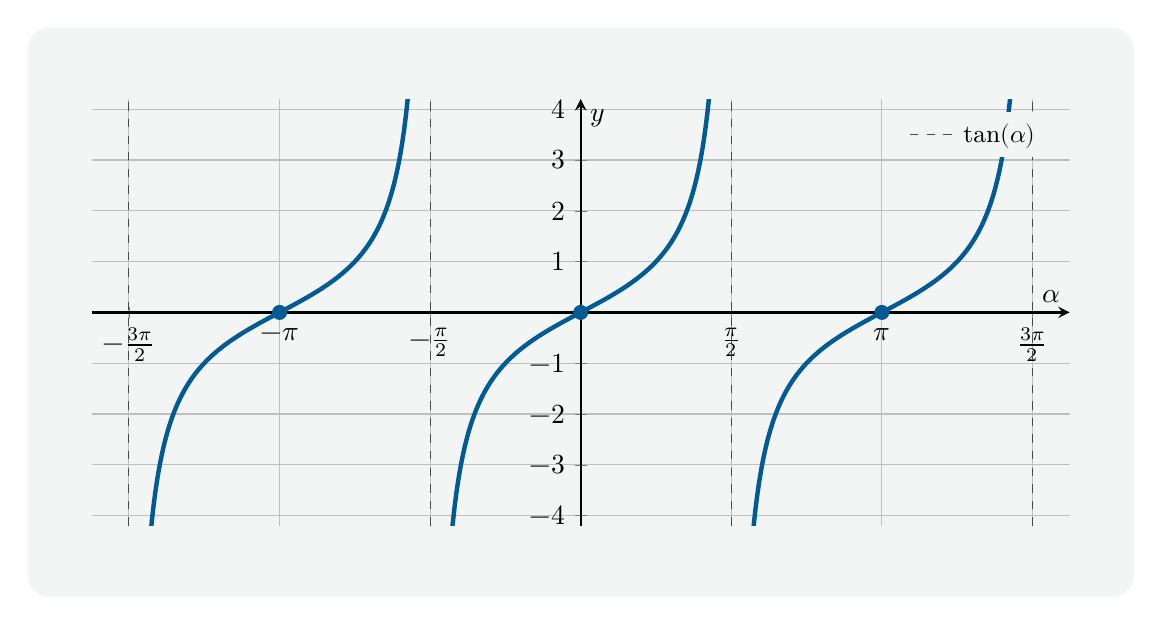
\begin{tikzpicture}[
    show background rectangle,
    background rectangle/.style={fill=my_lightgray, rounded corners=8pt},
    inner frame sep=0.8cm
]

\pgfmathsetmacro{\halfpi}{1.5708}
\pgfmathsetmacro{\threehalfpi}{4.7124}
\pgfmathsetmacro{\gap}{0.08}

\begin{axis}[
    axis lines=center,
    xlabel={$\alpha$},
    ylabel={$y$},
    height=7cm, width=14cm,
    xmin=-5.1, xmax=5.1,    % covers [-3pi/2-eps, 3pi/2+eps], i.e. 3 full periods
    ymin=-4.2, ymax=4.2,
    xtick={-4.7124, -3.1416, -1.5708, 0, 1.5708, 3.1416, 4.7124},
    xticklabels={
        $-\frac{3\pi}{2}$, $-\pi$, $-\frac{\pi}{2}$,
        $0$,
        $\frac{\pi}{2}$, $\pi$, $\frac{3\pi}{2}$
    },
    ytick={-4,-3,-2,-1,0,1,2,3,4},
    grid=both,
    axis line style={thick},
    restrict y to domain=-4.5:4.5,
    clip=true,
    legend style={
        font=\small,
        at={(0.98, 0.97)},
        anchor=north east,
        draw=none,
        fill=my_lightgray,
    },
    legend cell align=left,
]

% ── Vertical asymptotes drawn as individual \addplot vline commands ───────────
% Using \addplot coordinates with two points is the correct pgfplots idiom;
% \draw with axis cs: inside \foreach is unreliable inside an axis environment.
\addplot[dashed, my_darkgray, thin] coordinates {(-4.7124,-4.2) (-4.7124, 4.2)};
\addplot[dashed, my_darkgray, thin] coordinates {(-1.5708,-4.2) (-1.5708, 4.2)};
\addplot[dashed, my_darkgray, thin] coordinates {( 1.5708,-4.2) ( 1.5708, 4.2)};
\addplot[dashed, my_darkgray, thin] coordinates {( 4.7124,-4.2) ( 4.7124, 4.2)};

% ── Tangent branches ──────────────────────────────────────────────────────────

% Branch 1: (-3pi/2, -pi/2)
\addplot[draw=my_darkblue, samples=300, ultra thick,
         domain={-\threehalfpi+\gap}:{-\halfpi-\gap}]
    {tan(deg(x))};

% Branch 2: (-pi/2, pi/2)
\addplot[draw=my_darkblue, samples=300, ultra thick,
         domain={-\halfpi+\gap}:{\halfpi-\gap}]
    {tan(deg(x))};
\addlegendentry{$\tan(\alpha)$}

% Branch 3: (pi/2, 3pi/2)
\addplot[draw=my_darkblue, samples=300, ultra thick,
         domain={\halfpi+\gap}:{\threehalfpi-\gap}]
    {tan(deg(x))};

% ── Mark zeros at alpha = -pi, 0, pi ─────────────────────────────────────────
\addplot[only marks, mark=*, mark size=2.5pt,
         draw=my_darkblue, fill=my_darkblue]
    coordinates{(-3.1416, 0) (0, 0) (3.1416, 0)};

\end{axis}
\end{tikzpicture}
\end{document}
